%\begin{titlepage}
\newpage
\pagestyle{empty}
Работа выполнена в Белорусском национальном техническом \linebreak университете

\vspace*{-4mm}
\begin{table*}[h!]
\hspace*{-4mm}
\begin{tabular}{p{65mm} p{94mm}}

{Научный руководитель} & {\textbf{ФАМИЛИЯ Имя Отчество}, доктор технических наук, профессор, профессор кафедры <<Ложки и молотки>> Белорусского национального технического университета} \tabularnewline 

~&~ \tabularnewline 

{Официальные оппоненты:} & \textbf{ФАМИЛИЯ Имя Отчество}, доктор технических наук, ведущий научный сотрудник, заместитель генерального директора Государственного предприятия <<Институт ПВТ \linebreak им.~Яндекса~С.~С.>>;
\tabularnewline 

~&~ \tabularnewline 

~ & \textbf{ФАМИЛИЯ Имя Отчество}, кандидат технических наук, доцент, заведующий кафедрой <<Вилки, ложки и решето>> УО~<<Гондурасский государственный технический университет >>
\tabularnewline 

~&~ \tabularnewline 

{Оппонирующая организация} & РУП~<<НАЗВАНИЕ>>

\end{tabular}
\end{table*}

\vspace*{-6mm}
Защита состоится
%<<\underline{~~~~~~}>> \underline{~~~~~~~~~~~~~~} 2019~г.
%в \underline{~~~~~~} часов
<<30>> февраля 2020~г.
в 10 часов
на заседании совета по защите диссертаций Д 00.00.00
при Белорусском государственном университете
по адресу: 220019, г.~Минск, пр-т~Франциска Скорины, 165, корп.~1, ауд.~1258,
тел. ученого секретаря \mbox{+375~17~000-00-00}.

С диссертацией можно ознакомиться в библиотеке Белорусского государственного университета.

Автореферат разослан <<\underline{~~~~~}>> \underline{~~~~~~~~~~~~~~} 2018~г.

\begin{table*}[h!]
\hspace*{-4mm}
\begin{tabular}{p{100mm} c r}
Ученый секретарь &
\multirow{3}*{{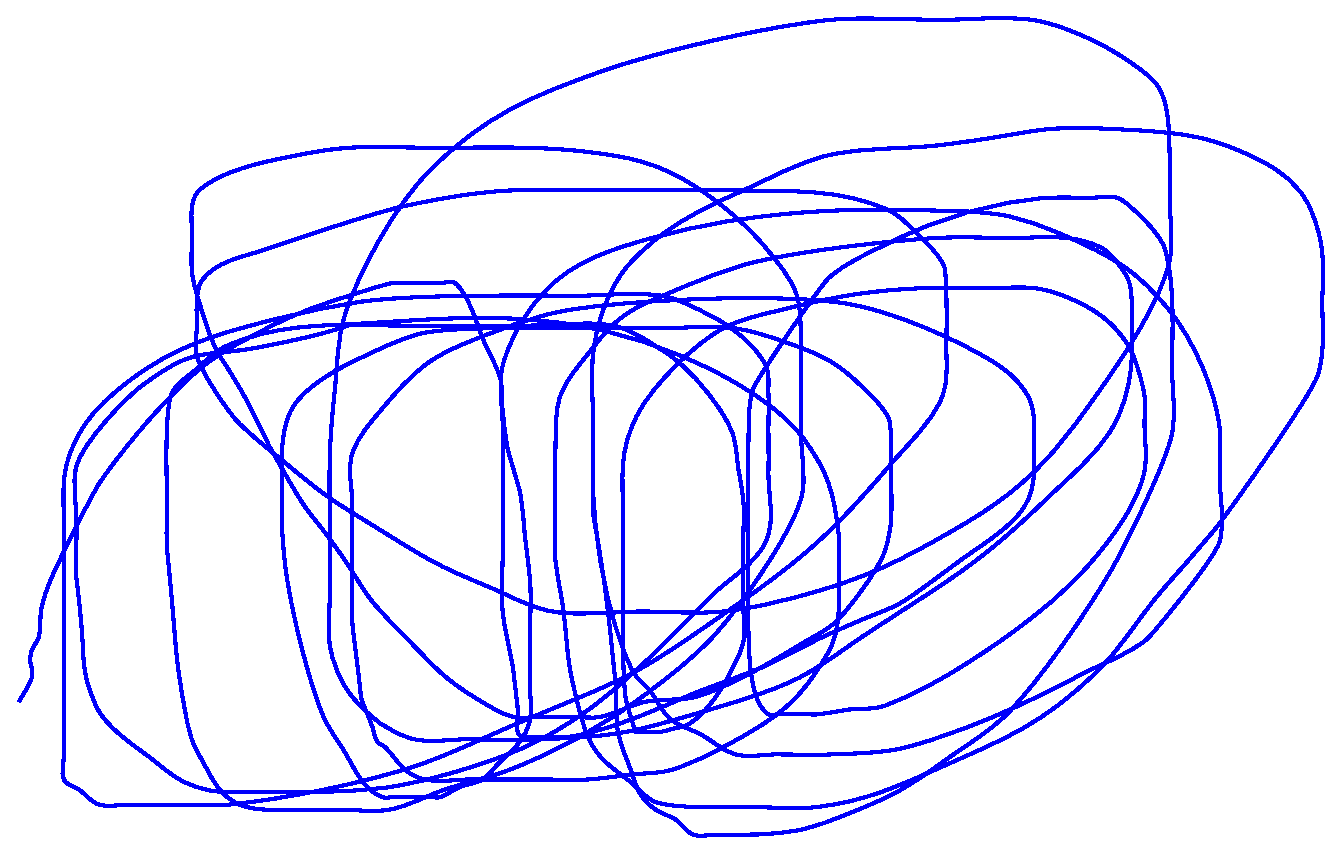
\includegraphics[width=3.5cm]{000sakratar_podpis}}}
&\\
совета по защите диссертаций, & &\\
доктор технических наук, профессор &  & И.~О.~Фамилия
\end{tabular}
\end{table*}
%
\vspace*{-3pt}
\begin{table*}[h!]
\hspace*{-4mm}
\begin{tabular}{p{80mm} l}
%
~ &  \copyright ~Вега~В.~Т., \the\year
\tabularnewline
~ & \copyright ~Белорусский национальный
\tabularnewline
~& ~~~~\,технический университет, \the\year
%
\end{tabular}
\end{table*}
%
%\end{titlepage}